% answers.tex —— 2006 年·全国卷Ⅰ·文科 · 参考答案与详细解析片段
% 由 tools/generate_projects.py 依来源总账自 2006/2006_数学真题_全国1文_试题.md + 2006/2006_数学真题_全国1文_解析正文.md + 2006/2006_数学真题_全国1文_答案要点.md 生成，勿手改（改源 MD 后重跑）


\begin{gktip}
固定源 PDF 为印刷页码 314–315 的两页题面，不附答案。以下解析均依据固定源独立复算；第 20 题图形在 LaTeX 工程中以 TikZ/PGFPlots 矢量源重绘。
\end{gktip}

\begin{answer}
\gksolhead{1}{}

\textbf{题目}：

已知向量 $\boldsymbol a,\boldsymbol b$ 满足 $|\boldsymbol a|=1$，$|\boldsymbol b|=4$，且 $\boldsymbol a\cdot\boldsymbol b=2$，则 $\boldsymbol a$ 与 $\boldsymbol b$ 夹角为\mbox{（　　）}

（A）$\dfrac\pi6$\quad（B）$\dfrac\pi4$\quad（C）$\dfrac\pi3$\quad（D）$\dfrac\pi2$

\Needspace{4\baselineskip}
\textbf{解析}

\nopagebreak[4]
\[
\cos\theta=\frac{\boldsymbol a\cdot\boldsymbol b}{|\boldsymbol a||\boldsymbol b|}=\frac{2}{1\cdot4}=\frac12,
\]

所以 $\theta=\dfrac\pi3$。

\gkanswer{答案：C}

\end{answer}
\begin{answer}
\gksolhead{2}{}

\textbf{题目}：

设集合 $M=\{x\mid x^2-x<0\}$，$N=\{x\mid |x|<2\}$，则\mbox{（　　）}

（A）$M\cap N=\varnothing$\quad（B）$M\cap N=M$\quad（C）$M\cup N=M$\quad（D）$M\cup N=\mathbb R$

\Needspace{4\baselineskip}
\textbf{解析}

由 $x^2-x<0$ 得 $0<x<1$，而 $0<x<1$ 蕴含 $|x|<2$，故 $M\subseteq N$，从而 $M\cap N=M$。

\gkanswer{答案：B}

\end{answer}
\begin{answer}
\gksolhead{3}{}

\textbf{题目}：

已知函数 $y=e^x$ 的图象与函数 $y=f(x)$ 的图象关于直线 $y=x$ 对称，则\mbox{（　　）}

（A）$f(2x)=e^{2x}\ (x\in\mathbb R)$\quad（B）$f(2x)=\ln2\cdot\ln x\ (x>0)$

（C）$f(2x)=2e^x\ (x\in\mathbb R)$\quad（D）$f(2x)=\ln x+\ln2\ (x>0)$

\Needspace{4\baselineskip}
\textbf{解析}

\Needspace{5\baselineskip}
$y=e^x$ 的反函数为 $y=\ln x\ (x>0)$，所以

\nopagebreak[4]
\[
f(2x)=\ln(2x)=\ln x+\ln2\quad(x>0)\text{。}
\]

\gkanswer{答案：D}

\end{answer}
\begin{answer}
\gksolhead{4}{}

\textbf{题目}：

双曲线 $mx^2+y^2=1$ 的虚轴长是实轴长的 $2$ 倍，则 $m=$\mbox{（　　）}

（A）$-\dfrac14$\quad（B）$-4$\quad（C）$4$\quad（D）$\dfrac14$

\Needspace{4\baselineskip}
\textbf{解析}

\Needspace{5\baselineskip}
双曲线要求 $m<0$。写成

\nopagebreak[4]
\[
y^2-(-m)x^2=1\text{，}
\]

\Needspace{5\baselineskip}
其实轴长分别为实轴 $2$、虚轴 $\dfrac{2}{\sqrt{-m}}$。由虚轴长为实轴长的 $2$ 倍，得

\nopagebreak[4]
\[
\frac{2}{\sqrt{-m}}=4\Longrightarrow m=-\frac14\text{。}
\]

\gkanswer{答案：A}

\end{answer}
\begin{answer}
\gksolhead{5}{}

\textbf{题目}：

设 $S_n$ 是等差数列 $\{a_n\}$ 的前 $n$ 项和，若 $S_7=35$，则 $a_4=$\mbox{（　　）}

（A）$8$\quad（B）$7$\quad（C）$6$\quad（D）$5$

\Needspace{4\baselineskip}
\textbf{解析}

\Needspace{5\baselineskip}
等差数列的前 $7$ 项关于第 $4$ 项对称，故

\nopagebreak[4]
\[
S_7=7a_4\text{，}
\]

于是 $a_4=5$。

\gkanswer{答案：D}

\end{answer}
\begin{answer}
\gksolhead{6}{}

\textbf{题目}：

函数 $f(x)=\tan\left(x+\dfrac\pi4\right)$ 的单调增区间为\mbox{（　　）}

（A）$\left(k\pi-\dfrac\pi2,k\pi+\dfrac\pi2\right)$，$k\in\mathbb Z$

（B）$(k\pi,(k+1)\pi)$，$k\in\mathbb Z$

（C）$\left(k\pi-\dfrac{3\pi}4,k\pi+\dfrac\pi4\right)$，$k\in\mathbb Z$

（D）$\left(k\pi-\dfrac\pi4,k\pi+\dfrac{3\pi}4\right)$，$k\in\mathbb Z$

\Needspace{4\baselineskip}
\textbf{解析}

\Needspace{5\baselineskip}
在 $\tan\left(x+\dfrac\pi4\right)$ 的定义域内导数为正，间断点为

\nopagebreak[4]
\[
x=\frac\pi4+k\pi\text{。}
\]

\Needspace{5\baselineskip}
因此单调增区间为

\nopagebreak[4]
\[
\left(k\pi-\frac{3\pi}4,k\pi+\frac\pi4\right)\text{，}\quad k\in\mathbb Z\text{。}
\]

\gkanswer{答案：C}

\end{answer}
\begin{answer}
\gksolhead{7}{}

\textbf{题目}：

从圆 $x^2-2x+y^2-2y+1=0$ 外一点 $P(3,2)$ 向这个圆作两条切线，则两切线夹角的余弦值为\mbox{（　　）}

（A）$\dfrac12$\quad（B）$\dfrac35$\quad（C）$\dfrac{\sqrt3}2$\quad（D）$0$

\Needspace{4\baselineskip}
\textbf{解析}

\Needspace{5\baselineskip}
圆心为 $O(1,1)$，半径为 $1$，且 $OP=\sqrt5$。设切点为 $T$，则 $PT=\sqrt{OP^2-OT^2}=2$。若两切线夹角为 $\theta$，则

\nopagebreak[4]
\[
\cos\frac\theta2=\frac{PT}{OP}=\frac2{\sqrt5},qquad
\cos\theta=2\cos^2\frac\theta2-1=\frac35\text{。}
\]

\gkanswer{答案：B}

\end{answer}
\begin{answer}
\gksolhead{8}{}

\textbf{题目}：

$\triangle ABC$ 的内角 $A,B,C$ 的对边分别为 $a,b,c$，若 $a,b,c$ 成等比数列，且 $c=2a$，则 $\cos B=$\mbox{（　　）}

（A）$\dfrac14$\quad（B）$\dfrac34$\quad（C）$\dfrac{\sqrt2}4$\quad（D）$\dfrac{\sqrt2}3$

\Needspace{4\baselineskip}
\textbf{解析}

\Needspace{5\baselineskip}
由等比关系 $b^2=ac$ 及 $c=2a$，得 $b^2=2a^2$。余弦定理给出

\nopagebreak[4]
\[
\cos B=\frac{a^2+c^2-b^2}{2ac}
=\frac{a^2+4a^2-2a^2}{4a^2}=\frac34\text{。}
\]

\gkanswer{答案：C}

\end{answer}
\begin{answer}
\gksolhead{9}{}

\textbf{题目}：

已知各顶点都在一个球面上的正四棱柱高为 $4$，体积为 $16$，则这个球的表面积是\mbox{（　　）}

（A）$16\pi$\quad（B）$20\pi$\quad（C）$24\pi$\quad（D）$32\pi$

\Needspace{4\baselineskip}
\textbf{解析}

\Needspace{5\baselineskip}
设正方形底面边长为 $s$，则 $s^2\cdot4=16$，故 $s=2$。正四棱柱的体对角线长为

\nopagebreak[4]
\[
\sqrt{s^2+s^2+4^2}=\sqrt{24}=2\sqrt6\text{。}
\]

球半径为 $\sqrt6$，所以球面面积为 $4\pi(\sqrt6)^2=24\pi$。

\gkanswer{答案：C}

\end{answer}
\begin{answer}
\gksolhead{10}{}

\textbf{题目}：

在 $\left(x-\dfrac1{2x}\right)^{10}$ 的展开式中，$x^4$ 的系数为\mbox{（　　）}

（A）$-120$\quad（B）$120$\quad（C）$-15$\quad（D）$15$

\Needspace{4\baselineskip}
\textbf{解析}

\Needspace{5\baselineskip}
通项中取 $k$ 个 $-\dfrac1{2x}$ 因子时幂次为 $10-2k$。令其等于 $4$，得 $k=3$，故 $x^4$ 的系数为

\nopagebreak[4]
\[
\binom{10}{3}\left(-\frac12\right)^3=-120\text{。}
\]

\gkanswer{答案：A}

\end{answer}
\begin{answer}
\gksolhead{11}{}

\textbf{题目}：

抛物线 $y=-x^2$ 上的点到直线 $4x+3y-8=0$ 距离的最小值是\mbox{（　　）}

（A）$\dfrac43$\quad（B）$\dfrac75$\quad（C）$\dfrac85$\quad（D）$3$

\Needspace{4\baselineskip}
\textbf{解析}

\Needspace{5\baselineskip}
抛物线上点 $(x,-x^2)$ 到直线的距离为

\nopagebreak[4]
\[
\frac{|4x-3x^2-8|}{5}
=\frac{3x^2-4x+8}{5},
\]

因为 $3x^2-4x+8>0$。二次式在 $x=\dfrac23$ 处取最小值 $\dfrac{20}{3}$，故距离最小值为 $\dfrac43$。

\gkanswer{答案：A}

\end{answer}
\begin{answer}
\gksolhead{12}{}

\textbf{题目}：

用长度分别为 $2,3,4,5,6$（单位：cm）的 $5$ 根细木棒围成一个三角形（允许连接，但不允许折断），能够得到的三角形的最大面积为\mbox{（　　）}

（A）$8\sqrt5\ \mathrm{cm}^2$\quad（B）$6\sqrt{10}\ \mathrm{cm}^2$\quad（C）$3\sqrt{55}\ \mathrm{cm}^2$\quad（D）$20\ \mathrm{cm}^2$

\Needspace{4\baselineskip}
\textbf{解析}

\Needspace{5\baselineskip}
五根木棒分成三组后，三边之和为 $20$。在固定周长下，三角形越接近等边，面积越大；由给定木棒能够得到的最均衡分组为 $6$、$7=2+5$、$7=3+4$。因此最大面积为

\nopagebreak[4]
\[
\sqrt{10(10-6)(10-7)(10-7)}=6\sqrt{10}\ \mathrm{cm}^2\text{。}
\]

\gkanswer{答案：B}

\end{answer}
\begin{answer}
\gksolhead{13}{}

\textbf{题目}：

已知函数 $f(x)=a-\dfrac1{2^x+1}$，若 $f(x)$ 为奇函数，则 $a=$\gkblank{}。

\Needspace{4\baselineskip}
\textbf{解析}

\Needspace{5\baselineskip}
奇函数满足 $f(0)=0$，于是

\nopagebreak[4]
\[
a-\frac12=0\text{，}\qquad a=\frac12\text{。}
\]

代回可验证 $f(-x)=-f(x)$。

\gkanswer{答案：$\dfrac12$}

\end{answer}
\begin{answer}
\gksolhead{14}{}

\textbf{题目}：

已知正四棱锥的体积为 $12$，底面对角线长为 $2\sqrt6$，则侧面与底面所成的二面角等于\gkblank{}。

\Needspace{4\baselineskip}
\textbf{解析}

\Needspace{5\baselineskip}
底面对角线为 $2\sqrt6$，所以底面面积为 $\dfrac{(2\sqrt6)^2}{2}=12$。由体积公式得高 $h=3$。底面中心到边的距离为 $\sqrt3$，设侧面斜高为 $l$，则

\nopagebreak[4]
\[
l=\sqrt{3^2+(\sqrt3)^2}=2\sqrt3\text{。}
\]

侧面与底面所成角 $\theta$ 满足 $\tan\theta=\dfrac3{\sqrt3}=\sqrt3$，故 $\theta=\dfrac\pi3$。

\gkanswer{答案：$\dfrac\pi3$}

\end{answer}
\begin{answer}
\gksolhead{15}{}

\textbf{题目}：

\Needspace{5\baselineskip}
设 $z=2y-x$，式中变量 $x,y$ 满足下列条件：

\nopagebreak[4]
\[
\begin{cases}
2x-y\geqslant-1,\\
3x+2y\leqslant23,\\
y\geqslant1,
\end{cases}
\]

则 $z$ 的最大值为\gkblank{}。

\Needspace{4\baselineskip}
\textbf{解析}

可行域的三个顶点为 $(0,1),(7,1),(3,7)$。目标函数 $z=2y-x$ 在这些点的值分别为 $2,-5,11$，所以最大值为 $11$。

\gkanswer{答案：$11$}

\end{answer}
\begin{answer}
\gksolhead{16}{}

\textbf{题目}：

安排 $7$ 位工作人员在 $5$ 月 $1$ 日至 $5$ 月 $7$ 日值班，每人值班一天，其中甲、乙二人都不安排在 $5$ 月 $1$ 日和 $2$ 日，不同的安排方法共有\gkblank{}种。（用数字作答）

\Needspace{4\baselineskip}
\textbf{解析}

\Needspace{5\baselineskip}
甲、乙只能安排在第 $3$ 至第 $7$ 日，先安排这两人有 $5\times4$ 种；其余 $5$ 人任意排列在剩下的日期，有 $5!$ 种。因此总数为

\nopagebreak[4]
\[
5\times4\times5!=2400\text{。}
\]

\gkanswer{答案：$2400$}

\end{answer}
\begin{answer}
\gksolhead{17}{}

\textbf{题目}：

已知 $\{a_n\}$ 为等比数列，$a_3=2$，$a_2+a_4=\dfrac{20}{3}$，求 $\{a_n\}$ 的通项公式。

\Needspace{4\baselineskip}
\textbf{解析}

\Needspace{5\baselineskip}
设公比为 $q$。由 $a_3=2$，有 $a_2=\dfrac2q,a_4=2q$，于是

\nopagebreak[4]
\[
\frac2q+2q=\frac{20}{3}
\Longrightarrow 3q^2-10q+3=0\text{。}
\]

\Needspace{5\baselineskip}
故 $q=3$ 或 $q=\dfrac13$，相应通项为

\nopagebreak[4]
\[
a_n=2\cdot3^{n-3}\quad\text{\text{或}}\quad a_n=2\cdot3^{3-n}\text{。}
\]

\gkanswer{答案：$a_n=2\cdot3^{n-3}$ 或 $a_n=2\cdot3^{3-n}$。}

\end{answer}
\begin{answer}
\gksolhead{18}{}

\textbf{题目}：

$\triangle ABC$ 的三个内角为 $A,B,C$，求当 $A$ 为何值时，$\cos A+2\cos\dfrac{B+C}{2}$ 取得最大值，并求出这个最大值。

\Needspace{4\baselineskip}
\textbf{解析}

\Needspace{5\baselineskip}
由 $A+B+C=\pi$，令 $t=\dfrac A2$，则 $0<t<\dfrac\pi2$，且

\nopagebreak[4]
\[
\cos A+2\cos\frac{B+C}{2}
=\cos2t+2\sin t
=1-2\sin^2t+2\sin t
=\frac32-2\left(\sin t-\frac12\right)^2\text{。}
\]

因此当 $\sin t=\dfrac12$，即 $A=\dfrac\pi3$ 时取得最大值 $\dfrac32$。

\gkanswer{答案：$A=\dfrac\pi3$ 时取得最大值，最大值为 $\dfrac32$。}

\end{answer}
\begin{answer}
\gksolhead{19}{}

\textbf{题目}：

$A,B$ 是治疗同一种疾病的两种药，用若干试验组进行对比试验。每个试验组由 $4$ 只小白鼠组成，其中 $2$ 只服用 A，另 $2$ 只服用 B，然后观察疗效。若在一个试验组中，服用 A 有效的小白鼠的只数比服用 B 有效的多，就称该试验组为甲类组。设每只小白鼠服用 A 有效的概率为 $\dfrac23$，服用 B 有效的概率为 $\dfrac12$。

（1） 求一个试验组为甲类组的概率；

（2） 观察 $3$ 个试验组，求这 $3$ 个试验组中至少有一个甲类组的概率。

\Needspace{4\baselineskip}
\textbf{解析}

\gksubpart{(1)}

\Needspace{5\baselineskip}
设一个试验组中 A 药有效的小白鼠数为 $X$，B 药有效数为 $Y$。则

\nopagebreak[4]
\[
P(X=0,1,2)=\left(\frac19,\frac49,\frac49\right)\text{，}\qquad
P(Y=0,1,2)=\left(\frac14,\frac12,\frac14\right)\text{。}
\]

\Needspace{5\baselineskip}
甲类组要求 $X>Y$，所以

\nopagebreak[4]
\[
p=P(Y=0)P(X\geqslant1)+P(Y=1)P(X=2)
=\frac14\cdot\frac89+\frac12\cdot\frac49=\frac49\text{。}
\]

\gksubpart{(2)}

\Needspace{5\baselineskip}
三个试验组相互独立，至少一个为甲类组的概率为

\nopagebreak[4]
\[
1-(1-p)^3=1-\left(\frac59\right)^3=\frac{604}{729}\text{。}
\]

\gkanswer{答案（1）：$\dfrac49$。}

\gkanswer{答案（2）：$\dfrac{604}{729}$。}

\end{answer}
\begin{answer}
\gksolhead{20}{}

\textbf{题目}：

如图，$l_1,l_2$ 是互相垂直的异面直线，$MN$ 是它们的公垂线段。点 $A,B$ 在 $l_1$ 上，$C$ 在 $l_2$ 上，$AM=MB=MN$。
\nopagebreak[4]
\begin{center}% 2006 年全国卷Ⅰ文科第 20 题：互相垂直的异面直线
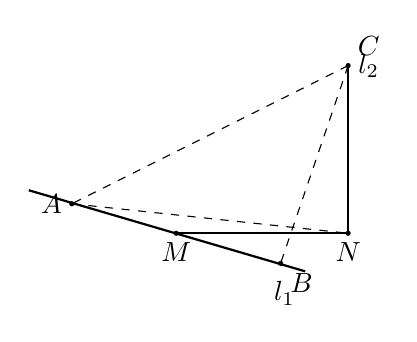
\begin{tikzpicture}[>=stealth,scale=0.78]
  \coordinate (A) at (0.55,1.20);
  \coordinate (M) at (2.25,0.72);
  \coordinate (B) at (3.95,0.23);
  \coordinate (N) at (5.05,0.72);
  \coordinate (C) at (5.05,3.45);
  \draw[thick] (-0.15,1.42)--(4.35,0.10) node[below left] {$l_1$};
  \draw[thick] (N)--(C) node[right] {$l_2$};
  \draw[thick] (M)--(N);
  \draw[dashed] (A)--(N) (C)--(A) (C)--(B);
  \fill (A) circle (1.2pt) node[left] {$A$};
  \fill (M) circle (1.2pt) node[below] {$M$};
  \fill (N) circle (1.2pt) node[below] {$N$};
  \fill (B) circle (1.2pt) node[below right] {$B$};
  \fill (C) circle (1.2pt) node[above right] {$C$};
\end{tikzpicture}
\end{center}
\nopagebreak[4]
（1） 证明：$AC\perp NB$；

（2） 若 $\angle ACB=60^\circ$，求 $NB$ 与平面 $ABC$ 所成角的余弦值。

\Needspace{4\baselineskip}
\textbf{解析}

\Needspace{5\baselineskip}
取 $MN=1$，建立直角坐标系，使

\nopagebreak[4]
\[
M=(0,0,0),\quad N=(0,0,1),\quad
A=(-1,0,0),\quad B=(1,0,0),\quad C=(0,t,1)\text{。}
\]

其中 $l_1$ 为 $x$ 轴，$l_2$ 为过 $N$ 且平行于 $y$ 轴的直线。

\gksubpart{(1)}

\Needspace{5\baselineskip}
有

\nopagebreak[4]
\[
\overrightarrow{AC}=(1,t,1),\qquad \overrightarrow{NB}=(1,0,-1)\text{，}
\]

从而 $\overrightarrow{AC}\cdot\overrightarrow{NB}=1-1=0$，故 $AC\perp NB$。

\gksubpart{(2)}

\Needspace{5\baselineskip}
由 $\angle ACB=60^\circ$，

\nopagebreak[4]
\[
\cos60^\circ
=\frac{\overrightarrow{CA}\cdot\overrightarrow{CB}}{|CA||CB|}
=\frac{t^2}{t^2+2}\text{，}
\]

\Needspace{5\baselineskip}
得 $t^2=2$。平面 $ABC$ 的一个法向量为

\nopagebreak[4]
\[
\boldsymbol n=\overrightarrow{AB}\times\overrightarrow{AC}=(0,-2,2t)\text{。}
\]

\Needspace{5\baselineskip}
设 $NB$ 与平面 $ABC$ 所成角为 $\theta$，则

\nopagebreak[4]
\[
\sin\theta=\frac{|\overrightarrow{NB}\cdot\boldsymbol n|}{|NB||\boldsymbol n|}
=\frac1{\sqrt3}\text{。}
\]

所以 $\cos\theta=\sqrt{\dfrac23}$。

\gkanswer{答案（1）：见解析版}

\gkanswer{答案（2）：$\sqrt{\dfrac23}$。}

\end{answer}
\begin{answer}
\gksolhead{21}{}

\textbf{题目}：

设 $P$ 是椭圆 $\dfrac{x^2}{a^2}+y^2=1\ (a>1)$ 短轴的一个端点，$Q$ 为椭圆上一个动点，求 $|PQ|$ 的最大值。

\Needspace{4\baselineskip}
\textbf{解析}

\Needspace{5\baselineskip}
不妨取短轴端点 $P=(0,1)$，令 $Q=(a\cos t,\sin t)$。则

\nopagebreak[4]
\[
|PQ|^2=a^2\cos^2t+(\sin t-1)^2\text{。}
\]

\Needspace{5\baselineskip}
令 $u=\sin t$，则 $-1\leqslant u\leqslant1$，并且

\nopagebreak[4]
\[
|PQ|^2=a^2+1-(a^2-1)u^2-2u\text{。}
\]

这是关于 $u$ 的开口向下的二次函数，其顶点为 $u_0=-\dfrac1{a^2-1}$。

\Needspace{5\baselineskip}
当 $1<a<\sqrt2$ 时，顶点在区间 $[-1,1]$ 左侧，最大值在 $u=-1$ 处取得，为 $4$；当 $a\geqslant\sqrt2$ 时，顶点在区间内，最大值为

\nopagebreak[4]
\[
a^2+1+\frac1{a^2-1}=\frac{a^4}{a^2-1}\text{。}
\]

\Needspace{5\baselineskip}
因此

\nopagebreak[4]
\[
|PQ|_{\max}=
\begin{cases}
2,&1<a<\sqrt2,\\[2pt]
\dfrac{a^2}{\sqrt{a^2-1}},&a\geqslant\sqrt2\text{。}
\end{cases}
\]

\gkanswer{答案：$2$（$1<a<\sqrt2$）；$\dfrac{a^2}{\sqrt{a^2-1}}$（$a\geqslant\sqrt2$）。}

\end{answer}
\begin{answer}
\gksolhead{22}{}

\textbf{题目}：

设 $a$ 为实数，函数 $f(x)=x^3-ax^2+(a^2-1)x$ 在 $(-\infty,0)$ 和 $(1,+\infty)$ 都是增函数，求 $a$ 的取值范围。

\Needspace{4\baselineskip}
\textbf{解析}

\nopagebreak[4]
\[
f'(x)=3x^2-2ax+a^2-1\text{。}
\]

在 $x<0$ 上考察这个二次式：若 $a\geqslant0$，其顶点不在该区间，最小值趋近于 $f'(0)=a^2-1$，故需 $a\geqslant1$；若 $a<0$，顶点 $x=a/3<0$，最小值为 $\dfrac{2a^2}{3}-1$，故需 $a\leqslant-\sqrt{\dfrac32}$。在 $x>1$ 上，若顶点不在区间则 $f'(1)=(a-1)^2+1>0$，若顶点在区间则其最小值为 $\dfrac{2a^2}{3}-1>0$，不再产生额外限制。

\Needspace{5\baselineskip}
所以

\nopagebreak[4]
\[
a\in\left(-\infty,-\sqrt{\frac32}\right]\cup[1,+\infty)\text{。}
\]

\gkanswer{答案：$a\in\left(-\infty,-\sqrt{\dfrac32}\right]\cup[1,+\infty)$。}

\end{answer}